%=========================================================================
% main_conf_EN.tex
% Traduccion al ingles de main_conf.tex, sobre el mismo template oficial de
% conferencia IEEE (conference_101719.tex / IEEEtran.cls).
%
% Diferencias respecto de main_conf.tex:
%   - babel pasa de [spanish,es-tabla,es-noquoting] a [english]: cambia la
%     hifenacion y los nombres automaticos (Table, Fig., etc.).
%   - El signo de porcentaje va pegado al numero (54%), que es la convencion
%     tipografica inglesa; en espanol iba separado (54 %).
%   - Los comentarios del fuente se mantienen en espanol.
% Estructura, ecuaciones, tablas, figuras, numeros y bibliografia son
% identicos a main_conf.tex. Cualquier cambio de contenido debe hacerse en
% ambos archivos.
%=========================================================================
\documentclass[conference]{IEEEtran}
\IEEEoverridecommandlockouts
% The preceding line is only needed to identify funding in the first footnote. If that is unneeded, please comment it out.
\usepackage{cite}
\usepackage{amsmath,amssymb,amsfonts}
\usepackage{algorithmic}
\usepackage{graphicx}
\usepackage{textcomp}
%\usepackage{xcolor}
\def\BibTeX{{\rm B\kern-.05em{\sc i\kern-.025em b}\kern-.08em
    T\kern-.1667em\lower.7ex\hbox{E}\kern-.125emX}}

% ------------------- Agregados requeridos por el contenido ---------------
\usepackage{lmodern}                 % fuentes T1 escalables
\usepackage[T1]{fontenc}
\usepackage[utf8]{inputenc}
\usepackage[english]{babel}          % paper en ingles
\usepackage{array}                   % columnas de las tablas
\usepackage{booktabs}                % \toprule, \midrule, \bottomrule
\usepackage[table]{xcolor}           % \rowcolor en las tablas
\usepackage{stfloats}                % figure* al pie de pagina
\usepackage{subcaption}              % paneles (a)/(b) de las figuras
\usepackage{tikz}                    % Fig. del esquema de implementacion
\usepackage{comment}
\usetikzlibrary{arrows.meta,positioning,calc,decorations.pathmorphing}

% ---------------------------- Definiciones ------------------------------
\newcommand{\gv}{\boldsymbol{\gamma}}
\newcommand{\av}{\boldsymbol{\alpha}}

% Simbolo de porcentaje valido en texto y en modo matematico. Se conserva de
% main_conf.tex para que ambas versiones rindan identico.
\newcommand{\pct}{\text{\char`\%}}

\definecolor{Gray}{gray}{0.9}   % 0 = black, 1 = white

\graphicspath{{Figures/}}

%=========================================================================
\begin{document}

\title{
%Multipolar OPP Modulation in Grid-Connected T-Type Converters with Loss Reduction and TDD Constraints
Loss-Minimizing Multipolar Optimal Pulse Patterns for Grid-Connected T-Type Converters With IEEE~519 Compliance
%Multipolar OPP Modulation in Grid-Connected T-Type Converters with Loss Reduction and TDD Constraints
%Multipolar OPP Modulation in T-Type Converters for Grid-Tied Systems with Loss Reduction and TDD Constraints
%Multipolar OPP Modulation in T-Type Converters for Grid Power Injection with Loss Reduction and TDD Constraints

%\thanks{Identify applicable funding agency here. If none, delete this.}
}

%\author{\IEEEauthorblockN{Carlos Stappung}
%\IEEEauthorblockA{\textit{Department of Electrical Engineering} \\
%\textit{UC Energy Research Center} \\
%\textit{Solar Energy Research Center} \\
%\textit{Pontificia Universidad Católica de Chile}\\
%Santiago, Chile \\
%carlos.stappung@uc.cl}
%\and
%\IEEEauthorblockN{Javier Pereda}
%\IEEEauthorblockA{\textit{Department of Electrical Engineering} \\
%\textit{UC Energy Research Center} \\
%\textit{Solar Energy Research Center} \\
%\textit{Pontificia Universidad Católica de Chile}\\
%Santiago, Chile \\
%https://orcid.org/0000-0002-3407-5233}}



\maketitle

% ------------------------------ Abstract --------------------------------
\begin{abstract}
In grid-connected converters operating at low switching frequency,
carrier-based modulation schemes degrade the quality of the injected current.
This paper presents a multipolar optimal pulse pattern (OPP) formulation for a
three-level SiC T-Type inverter that directly minimizes the converter losses
subject to the total demand distortion (TDD) limit of the IEEE~519 standard.
Conduction and switching loss models are derived as a function of the virtual
angles, so far unavailable for this topology, and the integer level constraint
is replaced by linear inequalities, yielding a continuous nonlinear problem.
Simulation results show reductions of the total losses at the nominal operating
point of 56\pct{} with respect to DPWM1 at 6450~Hz and 40\pct{} with respect to
PWM at 2850~Hz, with comparable conduction losses and compliance with the
standard over the entire power range.
\end{abstract}

\begin{IEEEkeywords}
Optimal pulse pattern, multipolar modulation, T-Type converter, virtual angle,
loss minimization, IEEE~519.
\end{IEEEkeywords}

% ============================ S1 ========================================
\section{Introduction}

In high-power conversion systems, the high blocking voltages and switched
currents make conduction and switching losses significant
\cite{zhang_hpm,edpuganti_survey}. Two fronts are available to mitigate them:
the topology and device selection, and the modulation technique. This work
addresses both, in that order.

On the first front, the three-level T-Type with SiC devices is adopted. The
neutral-point-clamped (NPC) converter is the reference topology for improving the
output waveform and limiting the filter size \cite{lee_npc_ttype}, but the T-Type
achieves the same number of levels with fewer semiconductors in the conduction
path, which at low switching frequency translates into lower total losses
\cite{alemi_ttype}. The break-even point between the two lies between 10 and
15~kHz and shifts upwards with SiC, whose switching energies are much lower than
those of an equivalent IGBT \cite{yang_sic_gan}: the thermal balance tilts
towards conduction, which is where the T-Type outperforms the NPC. Restricting
the modulation to single-level transitions, forbidding the direct step between
$+1$ and $-1$, makes every transistor switch while blocking half of the DC link,
so that the switching losses match those of the NPC and the conduction advantage
is preserved. The usual objection, that $S_1$ and $S_4$ must withstand the full
DC link, only matters when the link voltage exceeds what a single device can block
and forces the use of devices in series: with 750~V DC and 1.2~kV SiC MOSFETs a single
device blocks it with margin, and the growing availability of higher-voltage SiC
devices \cite{narasimhan_sic,nielsen_10kv} extends the argument to higher
voltages.

Modulation techniques are grouped into carrier-based, space-vector and
programmed schemes. The first two are well suited to medium-to-high switching
frequency range, but in high-power converters, which operate at low frequencies
to limit their losses, they generate low-order harmonics and degrade the current
quality. Given this limitation, programmed modulation, and in particular the
optimal pulse pattern (OPP), becomes competitive \cite{zhang_hpm}.

The generalized OPP proposed in \cite{birth_genopp} removes the constraint that
restricts switching to positive transitions during the positive half-cycle and
to negative ones during the negative half-cycle. This formulation, known as
multipolar modulation, significantly enlarges the feasible space and enables TDD
reductions of up to one third with respect to the traditional formulation for
the same number of angles. That additional margin can be reinvested in
minimizing losses while keeping the TDD within the regulatory limit. In
addition, the virtual angle concept \cite{koukoula_junction} eliminates the
integer variables associated with the switching positions, reducing the
computational cost of the optimization. This cost is precisely the main barrier
to the industrial adoption of the OPP \cite{zhang_hpm}; among the alternatives
under development, artificial neural networks stand out
\cite{filho_ann,ibanez_ann}, able to generate the patterns online after a
demanding off-line training. This work, in contrast, seeks to simplify the
model to keep the computational cost low.

The trade-off between distortion and losses is well documented for three-level
converters: detailed NPC versus T-Type comparisons are available
\cite{lee_npc_ttype,alemi_ttype} and, for the NPC, OPP formulations that model
the losses as a function of the angles \cite{koukoula_junction}. No T-Type loss
model expressed as a function of the angles and embedded in the optimization has
been reported, however, and even less so with SiC devices, whose split between
conduction and switching differs from that of an IGBT. Unity power factor at the point of common coupling is assumed over the whole
operating range.

The contributions of this work are the following:
\begin{itemize}
    \item An analytical conduction and switching loss model for the three-level
    T-Type with SiC devices, expressed directly as a function of the virtual
    angles and therefore continuous and differentiable.
    \item A multipolar OPP formulation with half-wave symmetry in which the
    integer level constraint is replaced by two linear inequalities on the
    angles.
    %\item The incorporation of the LCL filter through an explicit constraint on
    %the capacitor current, required for the loss model to be consistent with the
    %actual operation of the converter.
\end{itemize}

% La figura de la topologia se cita en la introduccion y en la Seccion de
% perdidas; se ancla aqui para que flote a la pagina siguiente al titulo.
% A una columna los rotulos S1..S4 quedan ilegibles (la figura tiene relacion de
% aspecto 3.5:1 con tres paneles), por eso va a dos columnas.
\begin{figure*}[!t]
    \centering
    \includegraphics[width=0.95\textwidth]{Figures/Topologia_T_Type.pdf}
    \caption{Three-level T-Type topology and per-leg conduction states: P, O and
    N. The conduction path of the current in each state is highlighted in red.}
    \label{fig:ttype}
\end{figure*}

% ============================ S3 ========================================
\section{Multipolar Harmonic Formulation}

This section poses the multipolar pattern as a continuous optimization variable:
the symmetry is chosen first, the Fourier coefficients are then written in terms
of the virtual angle, and finally the integer level constraint is replaced by
linear inequalities on the angles.

\subsection{Multipolar Modulation and Choice of Symmetry}

Half-wave symmetry (HWS) is adopted over quarter-wave symmetry (QWS). QWS
enforces symmetry between half-cycles and restricts the search space, preventing
the lower-distortion multipolar solutions reported in \cite{birth_genopp} from
being reached; the full-wave alternative is discarded because it admits a DC
component, which would compromise the neutral-point balance. HWS doubles the
number of variables to $2d$ angles, its only drawback, without altering the
structure of the problem or introducing additional constraints.

\subsection{Virtual Angle and Fourier Coefficients}

The standard formulation mixes continuous angles $\alpha_i$ with integer
positions $u_i \in \{-1,0,1\}$, resulting in a mixed-integer problem that is
difficult to solve. The virtual angle
$\gamma_i = \alpha_i + \frac{1-\Delta u_i}{2}\pi$ encodes the sign of the step in
its position: positive if $\gamma_i < \pi$, negative if $\gamma_i \geq \pi$. With
it, the Fourier coefficients under HWS, which contain only odd harmonics, reduce
to \eqref{eq:fourier_gamma}, free of integer variables.
\begin{equation}
    a_n = -\frac{2}{n\pi}\sum_{i=1}^{2d}\sin(n\gamma_i), \quad
    b_n =  \frac{2}{n\pi}\sum_{i=1}^{2d}\cos(n\gamma_i),
    \label{eq:fourier_gamma}
\end{equation}
thereby eliminating the integer variable $\Delta u_i \in \{-1,+1\}$ and turning
the problem into a continuous nonlinear one, suitable for local solvers. The
amplitude of the $n$-th harmonic of the output voltage is
$\hat{v}_n = \frac{V_{dc}}{2}\sqrt{a_n^2+b_n^2}$ and the current TDD, normalized
with respect to $I_{nom}$, is
\begin{equation}
    I_{TDD} = \frac{100\pct}{I_{nom}}
              \sqrt{\sum_{n=5,7,\dots} \left(\hat{v}_n\,g_n\right)^2}
    \label{eq:tdd}
\end{equation}
where $g_n$ is the transfer function of the LCL filter, from converter voltage to grid current, evaluated at harmonic $n$ (Section~\ref{sec:filtro}).

\subsection{Linear Level Constraints}
Even when the virtual angle is used, the model in \cite{koukoula_junction}
retains an integer level constraint, $-1 \leq u_i \leq 1$, which requires the
switching positions to be reconstructed at every solver iteration. To remove it,
the following inequalities, which act directly on the angles, are proposed:
\begin{subequations}
     \begin{align}
        \gamma_{i+d} - \pi &\leq \gamma_{i+1}
            &&\forall i = 1,\dots,d-1\\
        \gamma_{i} &\leq \gamma_{i+d+1} - \pi
            &&\forall i = 1,\dots,d-1
    \end{align}
    \label{eq:niveles}
\end{subequations}
where $d$ is the number of pulses per half-cycle. The first prevents the maximum level
from being exceeded and the second the minimum level, so that the feasible set is
described exclusively by linear constraints on $\gv$.

% ============================ S4 ========================================
\section{Loss Estimation}
\label{sec:perdidas}

The objective function is the total converter loss, given by the sum of a conduction and a switching term. Both are derived below as closed-form functions
of the virtual angles, so that the optimizer can evaluate them and their
gradients without simulating the pattern at each iteration. The section closes
with the design of the LCL filter that couples the converter to the grid.

\subsection{Conduction Losses}

The three-level T-Type has three possible conduction states, summarized in
Table~\ref{tab:estados_cond} and illustrated in Fig.~\ref{fig:ttype}. Since the
devices employed are SiC MOSFETs, the conduction voltage is purely resistive
($v_T = r_{ds,on}\,i$), which allows the instantaneous dissipated power to be
expressed as
\begin{equation}
    p_{con}(\gamma) = r_{ds,on}\,i^2(\gamma)
                    = r_{ds,on}\,I^2\sin^2(\gamma-\varphi).
    \label{eq:p_con}
\end{equation}
where $\varphi$ is the displacement between the fundamental of the modulated
voltage and the converter current, which does not vanish under unity power
factor at the point of common coupling because of the LCL capacitor, and is
evaluated from the filter parameters at each operating point.
\begin{table}[!t]
    \centering
    \caption{Per-leg conduction states of the three-level T-Type.}
    \bgroup
    \def\arraystretch{1.0}
    \begin{tabular}{c c}         \toprule
            \rowcolor{Gray}
        State & Conducting devices \\ \midrule
        P & $S_1$ \\
        O & $S_2 + S_3$ \\
        N & $S_4$ \\
        \bottomrule
    \end{tabular}
    \egroup
    \label{tab:estados_cond}
\end{table}
The proposed formulation groups the virtual angles into pairs
$(\gamma_i,\gamma_{i+d})$. Between the two angles of a pair either $S_1$ or
$S_4$ conducts, but it is not possible to determine a priori which of the two is
larger, so the length of the interval must be taken in absolute value. For $S_2$
and $S_3$ the difficulty is different: the integration limits are not defined
beforehand. A decomposition strategy is therefore adopted: the losses are first
computed as if $S_2$ and $S_3$ conducted over the whole period, and the
contribution of the intervals in which they do not actually conduct is then
subtracted; these are precisely the intervals bounded by each pair $(\gamma_i,\gamma_{i+d})$ in Fig.~\ref{fig:patron_opp}. This
yields
\begin{equation}
    P_{cond,S2+S3} = P_{cond,S2+S3}^{full}
        - \sum_{i=1}^{d}\hat{p}_{S2+S3}(\gamma_i,\gamma_{i+d})
    \label{eq:pcond_s2s3}
\end{equation}
where each term of the sum is evaluated by Simpson's rule over the interval of
the pair,
\begin{multline}
    \hat{p}_{j}(\gamma_i,\gamma_{i+d}) =
    \frac{|\gamma_{i+d}-\pi-\gamma_i|}{6}
    \Bigg( p_{j,con}(\gamma_i)\\
    + 4\,p_{j,con}\!\left(\frac{\gamma_i+\gamma_{i+d}-\pi}{2}\right)
    + p_{j,con}(\gamma_{i+d}-\pi) \Bigg).
    \label{eq:simpson}
\end{multline}

The losses of $S_1$ and $S_4$ are integrated over those same intervals, but with
half the conduction resistance, since a single semiconductor conducts within
them. Adding both contributions, the total conduction losses become
\begin{multline}
    P_{cond} = P_{cond,S2+S3}^{full}
        - \sum_{i=1}^{d}\hat{p}_{S2+S3}(\gamma_i,\gamma_{i+d})\\
        + \sum_{i=1}^{d}\hat{p}_{S1\text{-}S4}(\gamma_i,\gamma_{i+d}).
    \label{eq:pcond_total}
\end{multline}
Over a given interval $\hat{p}_{S2+S3}$ is exactly twice
$\hat{p}_{S1\text{-}S4}$, so both sums are merged into one and the expression
reduces to
\begin{equation}
    P_{cond} = P_{cond,S2+S3}^{full} - \sum_{i=1}^{d}
        \hat{p}_{S1\text{-}S4}(\gamma_i,\gamma_{i+d}),
    \label{eq:pcond_final}
\end{equation}
where the first term is constant for a given current and the whole dependence on
$\gv$ is concentrated in the sum.

\begin{figure}[!t]
    \centering
    \includegraphics[width=0.95\linewidth]{figuras/diagrama_grid_0_pi/diagrama_grid_0_pi.png}
    \caption{Multipolar OPP pattern with $d=5$ over the first half-cycle. Opening angles $\gamma_i$ are shown in blue and closing angles $\gamma_{i+d}-\pi$ in red.}
    \label{fig:patron_opp}
\end{figure}

\subsection{Switching Losses}

Switching losses depend on the voltage and the current at the exact switching
instant. Since every transition is single-level, the switched voltage is always
$V_{dc}/2$. Table~\ref{tab:transiciones_zvs} summarizes, for positive phase
current, which device incurs a loss in each transition and which one switches at
zero voltage (zero voltage switching, ZVS). ZVS arises from the directionality
of the current: if at the firing instant it already flows through the
antiparallel diode, the diode keeps the switch voltage close to zero and the
transistor switches without losses. Moreover, the reverse recovery charge of the
SiC diode is negligible, so that both contributions approach zero.

\begin{table}[!t]
    \centering
    \caption{Switching transitions and ZVS conditions.}
    \bgroup
    \def\arraystretch{1.0}
    \begin{tabular*}{\columnwidth}{@{\extracolsep{\fill}}cccc@{}}
        \toprule
        \rowcolor{Gray}
        Transition & Condition & Lossy Sw & ZVS Sw \\
        \midrule
        $P \rightarrow 0$ & $I > 0$ & $S_1$ off & $S_3$ on \\
        $0 \rightarrow N$ & $I > 0$ & $S_2$ off & $S_4$ on \\
        $N \rightarrow 0$ & $I > 0$ & $S_2$ on  & $S_4$ off \\
        $0 \rightarrow P$ & $I > 0$ & $S_1$ on  & $S_3$ off \\
        \bottomrule
    \end{tabular*}
    \egroup
    \label{tab:transiciones_zvs}
\end{table}

In each transition only the device that switches under voltage contributes
losses, so it is enough to account for those events: one turn-on per $\gamma_i$
and one turn-off per $\gamma_{i+d}$. Since the phase current is sinusoidal, the switched current is proportional to $\sin(\gamma_i-\varphi)$ at turn-on and to $\sin(\gamma_{i+d}-\pi-\varphi)$ at
turn-off (Fig.~\ref{fig:patron_opp}), so that the switching power becomes
\begin{equation}
    P_{sw} = f_1\,I_{cond}\sum_{i=1}^{d}
        \Big( E_{on}\sin(\gamma_i-\varphi)
            + E_{off}\sin(\gamma_{i+d}-\pi-\varphi)\Big)
    \label{eq:p_sw}
\end{equation}
where $f_1$ is the fundamental frequency, which turns the energy dissipated per
period into power, $I_{cond}$ is the current amplitude corresponding to the
modulation index under consideration, and $E_{on}$, $E_{off}$ are the switching
energies from the datasheet of the SiC module, evaluated at the blocking voltage
and normalized per ampere. With this, \eqref{eq:p_sw} is continuous and
differentiable in $\gv$.
%Since $\gamma_{i+d} \in [\pi,2\pi]$, the term
%$\sin(\gamma_{i+d})$ is negative and the subtraction accumulates positive
%contributions, consistent with the physics of the process.

\begin{figure*}[!t]
  \centering
  \includegraphics[width=\textwidth]{figuras/esquema_control_OPP_v3/esquema_control_OPP_v3.png}
  \caption{Implementation scheme: $dq$ current control, polar conversion of the
  voltage reference into modulation index $M$ and phase $\varphi$, OPP angle LUT
  and pattern generation synchronized with the grid angle $\theta$ of the PLL.}
  \label{fig:control}
\end{figure*}

\subsection{LCL Filter}
\label{sec:filtro}

The LCL filter acts as the interface between the converter and the grid. Its
resonance frequency is
\begin{equation}
    f_{res} = \frac{1}{2\pi}\sqrt{\frac{L_1+L_2}{L_1L_2C}}.
    \label{eq:fres}
\end{equation}

The resonance was placed at $f_{res}=1050$~Hz (21st harmonic): being a multiple
of three it is necessarily zero in the three-phase modulated voltage and its
neighbors are even, so that the resonance falls in a clear region of the
spectrum. The
capacitor was chosen as small as possible in order to minimize the injected
reactive power, and $L_1=L_2$, the choice that for a given $f_{res}$ minimizes
the total inductance $L_1+L_2$ and with it the volume of the filter.

% ============================ S5 ========================================
\section{OPP Implementation Scheme}

The pattern is obtained off-line, by solving a nonlinear program for each
modulation index, and applied online through a lookup table. Both stages are
described next.

\subsection{Optimization Problem}

Gathering the previous models, the problem to be solved for each modulation
index $M$ is formulated as
\begin{subequations}
    \setlength{\jot}{0pt}
    \begin{align}
        \min_{\gv}\;\; & P_{tot}(\gv) = P_{cond}(\gv) + P_{sw}(\gv)\\
        \text{s.t.}\;\; & a_1(\gv) = 0, \qquad b_1(\gv) = M\\
        & \gamma_{i+d}-\pi \leq \gamma_{i+1}
            &&\hspace{-14mm}\forall i = 1,\dots,d-1\\
        & \gamma_{i} \leq \gamma_{i+d+1}-\pi
            &&\hspace{-14mm}\forall i = 1,\dots,d-1\\
        & 0 \leq \gamma_1 \leq \dots \leq \gamma_d \leq \pi\\
        & \pi \leq \gamma_{d+1} \leq \dots \leq \gamma_{2d} \leq 2\pi\\
        & I_{TDD}(\gv) \leq 5\pct\\
        & I_{n}(\gv) \leq I_{n}^{\text{lim}} &&\hspace{-14mm}\forall n \leq 50\\
        %& I_{C,n}(\gv) \leq 2\pct\,I_{nom} &&\hspace{-14mm}\forall n \leq 80\\
        & \left\|\gv(M)-\gv(M-\Delta M)\right\|_{\infty} \leq \delta
    \end{align}
    \label{eq:opp_propuesto}
\end{subequations}

The equalities fix the amplitude and the phase of the fundamental. The level
inequalities are \eqref{eq:niveles} and replace the integer constraint; the
ordering ones separate the angles by half-cycle and guarantee single-level
transitions. IEEE~519 is imposed in its two forms: the global 5\pct{} limit on the TDD and
the individual limits $I_{n}^{\text{lim}}$ up to $n=50$, both taken for a
short-circuit ratio $I_{sc}/I_{L} < 20$. The last
one enforces continuity with respect to $M$, required for Section~\ref{sec:implementacion}. The
parameters are summarized in Table~\ref{tab:parametros}.

\begin{table}[!t]
    \centering
    \caption{System parameters considered.}
    \bgroup
    \def\arraystretch{1.0}
    % \rowcolor desborda la columna por ~2.5pt con el \tabcolsep por defecto.
    \setlength{\tabcolsep}{4pt}
    \begin{tabular*}{\columnwidth}{@{\extracolsep{\fill}}lcr@{}}
        \toprule
        \rowcolor{Gray}
        Parameter & Symbol & Value \\ \midrule
        Rated power & $P_{nom}$ & 10 kW \\
        DC-link voltage & $V_{dc}$ & 750 V \\
        Pulses per half-cycle & $d$ & 17 \\
        Switching frequency per device & $f_{sw}$ & 850 Hz \\
        Filter inductances & $L_1 = L_2$ & 1 mH \\
        Filter capacitor & $C$ & 46 $\mu$F \\
        Resonance frequency & $f_{res}$ & 1050 Hz \\
        Regulatory limit & TDD & 5\pct{} \\
        Grid voltage (line-to-line/RMS) & $V_{LL}$ & 400 V \\
        Rated current & $I_{nom}$ & 20 A \\
        Fundamental frequency & $f_1$ & 50 Hz \\
        T-Type SiC module & --- & CHB011M12GM4T \\
        \bottomrule
    \end{tabular*}
    \egroup
    \label{tab:parametros}
\end{table}


\subsection{Bilinear Dynamic Model of the Fourier Coefficients}
\label{sec:bilinear}

The formulation \eqref{eq:opp_nuevo} yields, for each modulation index,
an optimal pulse pattern under nominal conditions. However, it is a
non-convex NLP whose online solution is not feasible. The source of this
computational burden is the Fourier coefficients
\eqref{eq:fourier_gamma}, which are static and nonlinear with respect to
$\gv$. Therefore, a pragmatic approach to alleviate this burden is to
simplify them.

To this end, the $i$-th virtual angle of the set $\gv$ is decomposed
into two terms,
\begin{equation}
    \gamma_i = \gamma^0_i + \Delta\gamma_i,
    \label{eq:split}
\end{equation}
where $\gamma^0_i$ is the nominal angle initialized from a LUT such as
those obtained by solving \eqref{eq:opp_nuevo} offline, and
$\Delta\gamma_i$ is an adjustment term. Applying the angle sum and
difference identities, the trigonometric expressions in
\eqref{eq:fourier_gamma} are separated as
\begin{subequations}
    \begin{align}
        \sin(n\gamma_i) &= \sin(n\gamma^0_i)\cos(n\Delta\gamma_i)
                          +\cos(n\gamma^0_i)\sin(n\Delta\gamma_i)\\
        \cos(n\gamma_i) &= \cos(n\gamma^0_i)\cos(n\Delta\gamma_i)
                          -\sin(n\gamma^0_i)\sin(n\Delta\gamma_i).
    \end{align}
    \label{eq:angle_identity}
\end{subequations}

If $\Delta\gamma_i$ is small, then $\cos(n\Delta\gamma_i)\approx1$ and
$\sin(n\Delta\gamma_i)\approx n\Delta\gamma_i$. Substituting these
approximations into \eqref{eq:angle_identity} yields an expression that
is linear with respect to $\Delta\gamma_i$ when $\gamma^0_i$ is held
constant,
\begin{subequations}
    \begin{align}
        \sin(n\gamma_i) &\approx \sin(n\gamma^0_i)
                          + n\cos(n\gamma^0_i)\,\Delta\gamma_i\\
        \cos(n\gamma_i) &\approx \cos(n\gamma^0_i)
                          - n\sin(n\gamma^0_i)\,\Delta\gamma_i.
    \end{align}
    \label{eq:small_angle}
\end{subequations}

A dynamic interpretation of \eqref{eq:small_angle} is a difference
equation, where $\Delta\gamma_{i,k}$ is a small linear update from
$\gamma^0_{i,k}$ that produces
\begin{equation}
    \gamma^0_{i,k+1} = \gamma^0_{i,k} + \Delta\gamma_{i,k}.
    \label{eq:difference_eq}
\end{equation}

Applying \eqref{eq:small_angle} to \eqref{eq:fourier_gamma}, the dynamic
expression of the Fourier coefficients of the $n$-th harmonic becomes
\begin{subequations}
    \begin{align}
        a_{n,k+1} &= a_{n,k}
            -\frac{2}{\pi}\sum^{2d}_{i=1}\cos(n\gamma^0_{i,k})\,
             \Delta\gamma_{i,k}\\
        b_{n,k+1} &= b_{n,k}
            -\frac{2}{\pi}\sum^{2d}_{i=1}\sin(n\gamma^0_{i,k})\,
             \Delta\gamma_{i,k},
    \end{align}
    \label{eq:bilinear_scalar}
\end{subequations}
where $a_{n,k}$ and $b_{n,k}$ are evaluated at $\gv^0_k$ using
\eqref{eq:fourier_gamma}. Examining \eqref{eq:bilinear_scalar}, it is a
dynamic model that is linear with respect to $\Delta\gv_k$.

The constant terms and the coefficients in \eqref{eq:bilinear_scalar}
can be separated to obtain a more compact expression. Defining the
contribution of the $i$-th angle to the sum in \eqref{eq:fourier_gamma},
\begin{equation}
    a_{n,i} = -\frac{2}{n\pi}\sin(n\gamma^0_{i,k}),
    \qquad
    b_{n,i} = \frac{2}{n\pi}\cos(n\gamma^0_{i,k}),
    \label{eq:coef_i}
\end{equation}
and grouping the coefficients of the $n$-th harmonic into the vector
$\bm{x}_{n,k}=[a_{n,k}\;\;b_{n,k}]^{T}$, we obtain
\begin{equation}
    \bm{x}_{n,k+1} = \bm{x}_{n,k}
        + \bm{B}_{n,k}(\bm{x}_k)\cdot\Delta\gv_k,
    \label{eq:bilinear_n}
\end{equation}
where
\begin{equation}
    \bm{B}_{n,k}(\bm{x}_k) = n
    \begin{bmatrix}
        -b_{n,1} & \cdots & -b_{n,2d}\\
         a_{n,1} & \cdots &  a_{n,2d}
    \end{bmatrix}
    \in\mathbb{R}^{2\times2d}.
    \label{eq:Bn}
\end{equation}
The subscripts $k$ and $k+1$ are omitted in the expanded matrices for
notational brevity. Note that each column of $\bm{B}_{n,k}(\bm{x}_k)$
corresponds to the $i$-th virtual angle of the summation in
\eqref{eq:fourier_gamma}; hence the model is bilinear: it is linear in
$\Delta\gv_k$, but its coefficients depend on the linearization point
$\gv^0_k$ through $\bm{x}_k$.

Finally, \eqref{eq:bilinear_n} can be extrapolated up to the $N$-th
harmonic to obtain the complete bilinear dynamic model of the multilevel
pulse pattern,
\begin{equation}
    \underbrace{
    \begin{bmatrix} \bm{x}_{1,k+1}\\ \vdots\\ \bm{x}_{N,k+1}\end{bmatrix}
    }_{\bm{x}_{k+1}}
    =
    \underbrace{
    \begin{bmatrix} \bm{x}_{1,k}\\ \vdots\\ \bm{x}_{N,k}\end{bmatrix}
    }_{\bm{x}_{k}}
    +
    \underbrace{
    \begin{bmatrix} \bm{B}_{1,k}\\ \vdots\\ \bm{B}_{N,k}\end{bmatrix}
    }_{\bm{B}_{k}}
    \cdot
    \underbrace{
    \begin{bmatrix} {\Delta \gamma}_{1}\\ \vdots\\ {\Delta \gamma}_{2d}\end{bmatrix}
    }_{{\Delta \gamma}_{k}},
    \label{eq:bilinear_full}
\end{equation}
with $\bm{x}_k\in\mathbb{R}^{2N_{\text{mod}}}$ and
$\bm{B}_k\in\mathbb{R}^{2N_{\text{mod}}\times2d}$, where
$N_{\text{mod}}$ is the number of modeled harmonics. In this way, the
converter spectrum is described by a model that is linear with respect
to the virtual-angle adjustments, which enables the use of quadratic
programming in real time.

\subsection{Quadratic Program with Embedded Level Constraints}
\label{sec:qp}

The real-time adjustment of the pulse pattern then adopts the QP
formulation originally proposed by \cite{Tsekouras_RTlinear} for
three-level converters. The only structural difference introduced in
this work concerns the feasible set: in addition to the ascending order
of the switching angles, the multilevel-multipolar case additionally
requires the level constraints \eqref{eq:full_multipolar}. Since these
are inequality constraints, their real-time enforcement is imposed by
Dykstra's alternating projection algorithm
\cite{Dykstra_1983, Boyle_Dykstra_1986}, adopted precisely because this
method guarantees convergence to the projection onto any finite
intersection of closed convex sets. Consequently, the NLP model
\eqref{eq:opp_nuevo} is approximated by the QP
\begin{subequations}\label{eq:qp}
\begin{align}
\min_{\Delta\gv_k}\;&
      \underbrace{(\bm{x}^{\star} - \bm{x}_{k+1})^{T}\cdot\bm{Q}\cdot(\bm{x}^{\star} - \bm{x}_{k+1})}_{\text{WTHD}}
      +\lambda_u\cdot\underbrace{\Delta\gv_k^{T}\Delta\gv_k}_{\|\Delta\gv_k\|^2},
      \;\;,
      \label{eq:qp_cost}\\
\text{s.t.}\;& \gv^0_k+\Delta\gv_k \in \mathcal{F},
\label{eq:qp_feas}
\end{align}
\end{subequations}
where $\bm{x}_{k+1}$ is given by the bilinear model
\eqref{eq:bilinear_full} and $\mathcal{F}$ is the feasible set that
gathers the level constraints \eqref{eq:full_multipolar} and the
ordering constraints.

The WTHD term is responsible for the harmonic objective, where the
positive-definite diagonal matrix $\bm{Q}$ contains the weights $q_n$ of
each harmonic. Two classic choices are $\bm{Q}=\bm{I}$, which penalizes
the modeled harmonics equally (harmonic control), and $q_n=1/n^2$, which
minimizes the THD$_i$ as an OPP. The second term, weighted by
$\lambda_u$, penalizes the magnitude of the adjustments
$\|\Delta\gv_k\|^2$ to keep them small and thus preserve the validity of
the small-angle approximation \eqref{eq:small_angle}.

Consequently, \eqref{eq:bilinear_full} is first substituted into
\eqref{eq:qp_cost} and the gradient with respect to $\Delta\gv_k$ is set
to zero, which leads to the optimal analytic update policy
\begin{subequations}
\begin{align}
    \label{eq:analytic_update}
    \Delta\gv^{\text{unc}}_k = \bm{K}_k\big(\bm{x}^{\star}_k-\bm{x}_k\big),
    \;\;\\
    \bm{K}_k=\big(\bm{B}^{\mathsf T}_k\bm{Q}\bm{B}_k+\lambda_u\bm{I}\big)^{-1}
    \bm{B}^{\mathsf T}_k\bm{Q},
\end{align}
\end{subequations}
which requires solving a fixed-size linear system, and the adjusted
angles are then projected onto $\mathcal{F}$. Note that the term
$\lambda_u\bm{I}$ additionally guarantees that the matrix to be inverted
is positive definite, even when $\bm{B}_k$ is not of full column rank.

Dykstra's algorithm converges to the projection onto any finite
intersection of closed convex sets \cite{Bauschke_Borwein_1996}. Here,
$\mathcal{F}$ is split into four such sets: the maximum-level
constraints, the minimum-level constraints, the box
$0\leq\gamma_i\leq2\pi$, and the ordering cone. Each projection is
available in closed form. In particular, the constraints involving two
angles have a closed-form projection that distributes the violation
equally between the two angles involved. For a generic constraint of the
type $\gamma_a-\gamma_b\leq C$, \eqref{eq:proj_pair_le} is applied, and
for the complementary constraint $\gamma_a-\gamma_b\geq C$,
\eqref{eq:proj_pair_ge} is applied, where the violation is measured in
the opposite direction and the $\varepsilon/2$ adjustments reverse their
sign,
\begin{subequations}\label{eq:proj_pair}
\begin{align}
    \label{eq:proj_pair_le}
    \varepsilon &= \max\!\big(0,\;\gamma_a-\gamma_b-C\big),\;\;
    \gamma_a \leftarrow \gamma_a-\tfrac{\varepsilon}{2},\;\;
    \gamma_b \leftarrow \gamma_b+\tfrac{\varepsilon}{2},\\
    \label{eq:proj_pair_ge}
    \varepsilon &= \max\!\big(0,\;\ C - \gamma_a - \gamma_b \big),\;\;
    \gamma_a \leftarrow \gamma_a+\tfrac{\varepsilon}{2},\;\;
    \gamma_b \leftarrow \gamma_b-\tfrac{\varepsilon}{2}.
\end{align}
\end{subequations}
The maximum- and minimum-level constraints of \eqref{eq:full_multipolar}
are particular cases of \eqref{eq:proj_pair_le} and
\eqref{eq:proj_pair_ge}, respectively, with $C=\pi$; the box reduces to
a clipping and the ordering cone to a monotone sweep.

Consequently, each projection cycle involves only additions and
comparisons over at most two components at a time, without requiring
matrix factorization or branching over switching sequences. The pulse
pattern is thus kept within the limits while the computational cost
grows linearly with $d$. The proposed RT-ML-OPP is summarized in
Algorithm~\ref{alg:rtmlopp}, where, as in \cite{Tsekouras_RTlinear}, the
angles are adjusted sequentially.
\begin{equation}
    \gv^0_{k+1} \leftarrow \gv^{\text{opt}}_{k+1},
    \label{eq:sequential}
\end{equation}

\begin{algorithm}[!t]
\caption{RT-ML-OPP.}
\label{alg:rtmlopp}
\begin{algorithmic}[1]
\STATE \textbf{Given} $\bm{x}^{\star}_k$ and the initial point $\gv^0_k$
\STATE Form $\bm{x}_k$ and $\bm{B}_k$ from the bilinear dynamic model for
       the $N_{\text{mod}}$ harmonics linearized at $\gv^0_k$
\STATE Evaluate the optimal analytic update policy,
       $\Delta\gv^{\text{unc}}_k=\bm{K}_k\cdot(\bm{x}^{\star}_k-\bm{x}_k)$
\STATE Adjust the virtual angles from their initial point,
       $\gv_{k+1}=\gv^0_k+\Delta\gv^{\text{unc}}_k$
\STATE Enforce the level and ordering constraints by projecting
       $\gv_{k+1}$ onto $\mathcal{F}$
\STATE Recover $\av$ and $\Delta\bm{u}$ from $\gv^{\text{opt}}_{k+1}$;
       update the initial point,
       $\gv^0_{k+1}\leftarrow\gv^{\text{opt}}_{k+1}$
\end{algorithmic}
\end{algorithm}



\subsection{Control and Pattern Generation}
\label{sec:implementacion}

The off-line solution of \eqref{eq:opp_propuesto} is computed over the whole
operating range and stored as a lookup table (LUT) of angles $\gv(M)$,
according to the scheme of Fig.~\ref{fig:control}.


\begin{comment}
% requiere: \usetikzlibrary{arrows.meta}
\begin{figure*}[!t]
\centering
\resizebox{\textwidth}{!}{%
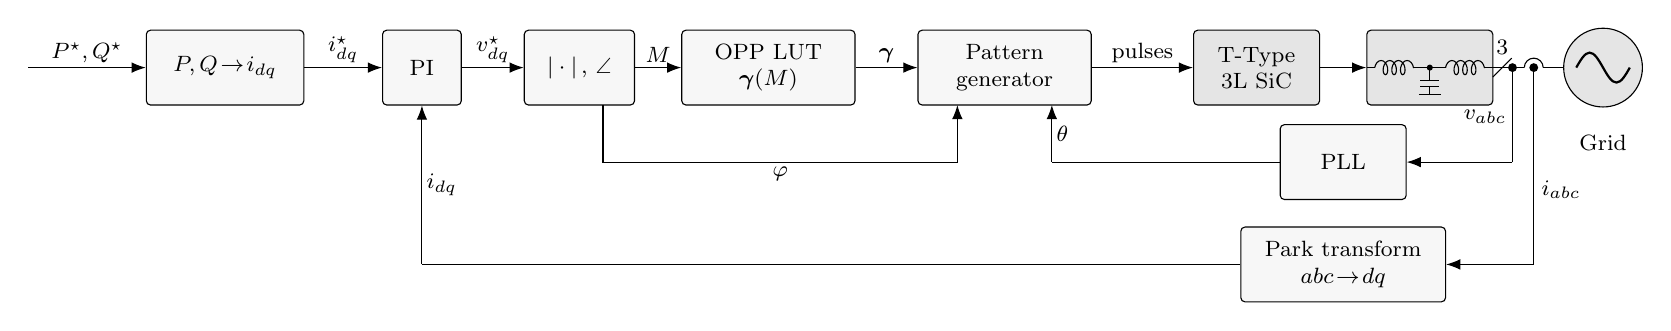
\begin{tikzpicture}[
  blk/.style={draw,rounded corners=1.5pt,minimum width=2.2cm,
              minimum height=0.95cm,align=center,font=\footnotesize,fill=black!3},
  pw/.style={draw,rounded corners=1.5pt,minimum width=1.6cm,
             minimum height=0.95cm,align=center,font=\footnotesize,fill=black!10},
  ln/.style={-{Latex[length=1.8mm]}},
  lbl/.style={font=\footnotesize,inner sep=1.5pt},
  coil/.style={decorate,decoration={coil,aspect=0.6,
               segment length=1.1mm,amplitude=0.9mm}}
]
% ---- main chain ----
\node[blk,minimum width=2.0cm] (ref) at (-3.6,0) {$P,Q\!\rightarrow\!i_{dq}$};
\node[blk,minimum width=1.0cm] (pi)  at (-1.1,0) {PI};
\node[blk,minimum width=1.4cm] (pol) at ( 0.9,0) {$|\cdot|\,,\,\angle$};
\node[blk,minimum width=2.2cm] (lut) at ( 3.3,0) {OPP LUT\\$\gv(M)$};
\node[blk,minimum width=2.2cm] (gen) at ( 6.3,0) {Pattern\\generator};
\node[pw,minimum width=1.6cm]  (conv)at ( 9.5,0) {T-Type\\3L SiC};
% ---- LCL filter symbol ----
\node[pw] (lcl) at (11.7,0) {};
\draw (10.9,0) -- (11.0,0);
\draw[coil] (11.0,0) -- (11.5,0);
\draw (11.5,0) -- (11.9,0);
\draw[coil] (11.9,0) -- (12.4,0);
\draw (12.4,0) -- (12.5,0);
\fill (11.7,0) circle (1.1pt);
\draw (11.7,0) -- (11.7,-0.16);
\draw (11.58,-0.16) -- (11.82,-0.16);
\draw (11.58,-0.24) -- (11.82,-0.24);
\draw (11.7,-0.24) -- (11.7,-0.34);
\draw (11.56,-0.34) -- (11.84,-0.34);
% ---- grid symbol (AC source) ----
\node[draw,circle,minimum size=1.0cm,inner sep=0pt,fill=black!10] (grid) at (13.9,0) {};
\draw[thick]
  ([xshift=-3.4mm]grid.center) sin ([xshift=-1.7mm,yshift=1.9mm]grid.center)
  cos (grid.center)            sin ([xshift= 1.7mm,yshift=-1.9mm]grid.center)
  cos ([xshift= 3.4mm]grid.center);
\node[lbl] at (13.9,-0.95) {Grid};
% ---- measurement and synchronisation ----
\node[blk,minimum width=1.6cm] (pll)  at (10.6,-1.2) {PLL};
\node[blk,minimum width=2.6cm] (meas) at (10.6,-2.5) {Park transform\\$abc\!\rightarrow\!dq$};
\coordinate (in) at (-6.1,0);
\draw[ln] (in)  -- node[lbl,above]{$P^{\star},Q^{\star}$} (ref);
\draw[ln] (ref) -- node[lbl,above]{$i_{dq}^{\star}$} (pi);
\draw[ln] (pi)  -- node[lbl,above]{$v_{dq}^{\star}$} (pol);
\draw[ln] (pol) -- node[lbl,above]{$M$} (lut);
\draw[ln] (lut) -- node[lbl,above]{$\gv$} (gen);
\draw[ln] (gen) -- node[lbl,above]{pulses} (conv);
\draw[ln] (conv) -- (lcl);
% ---- LCL -> grid line, interrupted at the current-measurement hop ----
\draw (lcl.east) -- (12.90,0);
\draw (13.14,0) -- (grid.west);
\draw ([shift={(-1.2mm,-1.2mm)}]12.62,0) -- ([shift={(1.2mm,1.2mm)}]12.62,0);
\node[lbl,above,inner sep=1pt] at (12.62,0.12) {3};
% ---- phi: polar block -> pattern generator (routed below) ----
\draw[ln] (1.2,-0.475) -- (1.2,-1.2)
          -- node[lbl,below]{$\varphi$} (5.7,-1.2) -- (5.7,-0.475);
% ---- voltage measurement (tap) -> PLL ----
\fill (12.75,0) circle (1.6pt);
\draw (12.75,0) -- (12.75,-1.2);
\draw[ln] (12.75,-1.2) -- (pll.east);
\node[lbl,left] at (12.73,-0.62) {$v_{abc}$};
% ---- current measurement: semicircular hop with centre dot ----
\draw (12.90,0) arc (180:0:0.12);
\fill (13.02,0) circle (1.6pt);
\draw (13.02,0) -- (13.02,-2.5);
\draw[ln] (13.02,-2.5) -- (meas.east);
\node[lbl,right] at (13.06,-1.55) {$i_{abc}$};
% ---- theta and measured currents ----
\draw (pll.west) -- (6.9,-1.2);
\draw[ln] (6.9,-1.2) -- node[lbl,right]{$\theta$} (6.9,-0.475);
\draw (meas.west) -- (-1.1,-2.5);
\draw[ln] (-1.1,-2.5) -- node[lbl,right]{$i_{dq}$} (pi.south);
\end{tikzpicture}}



\caption{Implementation scheme: $P,Q$ reference generation, $dq$ current PI control,
polar conversion of the voltage reference into modulation index $M$ and phase
$\varphi$, OPP angle LUT and pattern generation synchronized with the grid angle
$\theta$ provided by the PLL.}
\label{fig:control}
\end{figure*}
\end{comment}


The $dq$ power control provides the modulation index $M$ and the phase shift
$\varphi$. The LUT is addressed with $M$ and returns the angles; the pattern
generator converts them into firing instants synchronized with the grid angle
$\theta$ of the PLL.

A critical point of the scheme is the continuity of the LUT: the sets of optimal
solutions of an OPP exhibit discontinuities with respect to $M$, and an abrupt
jump in the angles translates into a current transient that the $dq$ controller
cannot compensate. Continuity is therefore not imposed a posteriori but within
the optimization itself, through the last constraint of
\eqref{eq:opp_propuesto}.


% =====================================================================
%  Real-Time Implementation -- Part 1: objective function
%  To be \input{} after Section~\ref{sec:implementacion} of main_conf_EN.tex
%  Uses the macros of the paper: \gv (boldsymbol gamma), \pct.
%  Notation follows RTOPP_D19.m (d = 19, N = 2d = 38, 17 harmonics).
% =====================================================================

\section{Real-Time Implementation}
\label{sec:rt}

The offline OPP of Section~\ref{sec:implementacion} is computed for a
discrete grid of operating points and stored in a LUT. Between grid
points, and whenever the grid voltage carries background distortion that
was not considered offline, the stored pattern is no longer optimal and may
even violate the harmonic limits. To address this, the angles are refined
online by a sequential quadratic program (SQP) executed once per control
period $T_s = 100~\mu$s. At each sample the harmonic spectrum and the loss
model are linearized around the current angles $\gv$, a single
Gauss--Newton (GN) step $\Delta\gv$ is computed, and the result is stored
as the warm start of the next sample. Convergence is therefore obtained
across samples rather than within one call, which bounds the computational
time per sample. The LUT, now indexed by the modulation index $M$ and the
load angle $\varphi$, provides only the initial pattern.

This subsection describes the objective function (OF) of the local problem;
the constraint handling is presented afterwards.
% TODO: \ref a la subseccion de restricciones cuando exista.

\subsection{Linearized Harmonic Model}
\label{subsec:rt_lin}

Under half-wave symmetry, $u(\theta+\pi) = -u(\theta)$, the pattern is
described by $N = 2d$ virtual angles
$\gv = [\gamma_1,\dots,\gamma_d,\gamma_{d+1},\dots,\gamma_{2d}]^T$: the
first $d$ are the rising steps within $[0,\pi)$, and the last $d$ are the
falling steps of the same half cycle shifted by $\pi$. Since a falling step
at $\theta$ produces, for odd $n$, the same harmonic as a rising step at
$\theta+\pi$, all $N$ angles contribute with the same sign:
%
\begin{equation}
  a_n = -\frac{2}{n\pi}\sum_{i=1}^{N}\sin(n\gamma_i), \qquad
  b_n =  \frac{2}{n\pi}\sum_{i=1}^{N}\cos(n\gamma_i),
  \label{eq:rt_anbn}
\end{equation}
%
for $n \in \mathcal{H} = \{1,5,7,11,13,\dots,49\}$, i.e., the odd,
non-triplen harmonics up to the 49th ($N_h = 17$). The spectrum vector is
$\mathbf{x} = [\mathbf{x}_1^T,\mathbf{x}_5^T,\dots]^T \in \mathbb{R}^{2N_h}$,
with $\mathbf{x}_h = [a_h,\, b_h]^T$. For a small increment,
%
\begin{equation}
  \mathbf{x}(\gv+\Delta\gv) \approx \mathbf{x}(\gv) + \mathbf{J}\,\Delta\gv,
  \label{eq:rt_lin}
\end{equation}
%
where the Jacobian $\mathbf{J}\in\mathbb{R}^{2N_h\times N}$ follows
exactly from \eqref{eq:rt_anbn}:
%
\begin{equation}
  \frac{\partial a_n}{\partial \gamma_i} = -\frac{2}{\pi}\cos(n\gamma_i),
  \qquad
  \frac{\partial b_n}{\partial \gamma_i} = -\frac{2}{\pi}\sin(n\gamma_i).
  \label{eq:rt_jac}
\end{equation}
%
Note that the $1/n$ factor cancels, so every harmonic is equally
sensitive to the angles in the spectral domain; the distinction between
harmonics is introduced by the weighting matrix below.

\subsection{TDD Term}
\label{subsec:rt_tdd}

Let $g_h$ be the grid-current amplitude produced by one unit of the
converter spectrum at harmonic $h$ through the LCL filter,
$g_h = (V_{dc}/2)\,|H_g(jh\omega_1)|$, and let $\mathbf{x}^\star$ be the
reference spectrum: $\mathbf{x}_1^\star = [0,\,M]^T$ for the fundamental
and, for $h\geq 5$, the background harmonics of the grid voltage expressed
in the same spectral units. The harmonic grid current is then proportional
to the mismatch $\mathbf{x}_h - \mathbf{x}_h^\star$, and the TDD reads
%
\begin{equation}
  \mathrm{TDD}(\gv) = \frac{100}{I_L}
  \sqrt{\sum_{h\in\mathcal{H},\,h\geq5} g_h^2\,
  \big\|\mathbf{x}_h(\gv)-\mathbf{x}_h^\star\big\|^2}\ \ [\pct].
  \label{eq:rt_tdd}
\end{equation}
%
With a clean grid, $\mathbf{x}_h^\star = \mathbf{0}$ for $h\geq5$ and
\eqref{eq:rt_tdd} reduces to the TDD definition used offline. Squaring
\eqref{eq:rt_tdd} gives a weighted quadratic form,
$\mathrm{TDD}^2 \propto \mathbf{x}_e^T\mathbf{Q}\,\mathbf{x}_e$ with
$\mathbf{x}_e = \mathbf{x}^\star - \mathbf{x}$ and the diagonal matrix
%
\begin{equation}
  \mathbf{Q} = \mathrm{diag}\big(q_1, q_1, q_5, q_5, \dots, q_{49}, q_{49}\big),
  \qquad
  q_h = w_{\mathrm{TDD}}\left(\frac{g_h}{I_L}\right)^{\!2}\!,\ h\geq 5.
  \label{eq:rt_Q}
\end{equation}
%
The weight $q_1 = 1$ only steers the GN step towards the desired
fundamental; the fundamental is imposed exactly as an equality constraint
afterwards. Because of the LCL resonance, $g_h$ peaks in the vicinity of
the 19th--23rd harmonics, so these entries of $\mathbf{Q}$ dominate the
TDD term.

\subsection{Loss Terms}
\label{subsec:rt_loss}

The loss model of Section~\ref{sec:implementacion} is extended with the
load angle $\varphi$, i.e., the phase current is
$i(\theta) = I_c\sin(\theta-\varphi)$, and all quantities are evaluated at
$\gamma_i - \varphi$.

\textit{Conduction:} define the primitive of $\sin^2\theta$,
$G(\theta) = \theta/2 - \sin(2\theta)/4$. For the $i$-th pulse, bounded by
the rising step $\gamma_i$ and the falling step $\gamma_{i+d}-\pi$, the
integral of the squared current is computed in closed form:
%
\begin{align}
  T_i(\gv) &= G(\gamma_{i+d}-\pi-\varphi) - G(\gamma_i-\varphi) \nonumber\\
           &= \frac{\gamma_{i+d}-\pi-\gamma_i}{2}
            - \frac{\sin 2(\gamma_{i+d}-\varphi) - \sin 2(\gamma_i-\varphi)}{4},
  \label{eq:rt_T}
\end{align}
%
for $i = 1,\dots,d$, which replaces the Simpson approximation of
\eqref{eq:simpson}. The conduction losses are
$P_{\mathrm{cond}} = I_c^2R_{on}\big(1 - \tfrac{1}{\pi}\sum_i T_i\big)$,
so reducing them amounts to enlarging the $T_i$. Their derivatives are
$\partial T_i/\partial\gamma_i = -\sin^2(\gamma_i-\varphi)$ and
$\partial T_i/\partial\gamma_{i+d} = \sin^2(\gamma_{i+d}-\varphi)$, hence
$\mathbf{T}(\gv+\Delta\gv) \approx \mathbf{T}^0 - \mathbf{B}_P\Delta\gv$
with
%
\begin{equation}
  \mathbf{B}_P = \Big[\ \mathrm{diag}\big(\sin^2(\gamma_i-\varphi)\big)
  \ \Big|\ -\mathrm{diag}\big(\sin^2(\gamma_{i+d}-\varphi)\big)\ \Big].
  \label{eq:rt_BP}
\end{equation}

\textit{Switching:} each pulse contributes a turn-on event at $\gamma_i$
and a turn-off event at $\gamma_{i+d}$. Using the magnitude of the
commutated current, so that no event can contribute negative energy,
%
\begin{equation}
  S_i(\gv) = E_{on}\,\big|\sin(\gamma_i-\varphi)\big|
           + E_{off}\,\big|\sin(\gamma_{i+d}-\varphi)\big|,
  \label{eq:rt_S}
\end{equation}
%
where $E_{on}$ and $E_{off}$ are the current-dependent energies per ampere,
corrected for the gate resistance $R_G$. The switching losses are
$P_{\mathrm{sw}} = P_{\mathrm{sw},0} + 2f_1I_c\sum_i S_i$, where
$P_{\mathrm{sw},0} = 2f_1d\,(E_{on,0}+E_{off,0})$ collects the
current-independent energies and does not depend on $\gv$. Linearizing,
$\mathbf{S}(\gv+\Delta\gv) \approx \mathbf{S}^0 - \mathbf{B}_S\Delta\gv$
with
%
\begin{equation}
  \mathbf{B}_S = -\Big[\ \mathrm{diag}\big(E_{on}\,c_i\,\sigma_i\big)
  \ \Big|\ \mathrm{diag}\big(E_{off}\,c_{i+d}\,\sigma_{i+d}\big)\ \Big],
  \label{eq:rt_BS}
\end{equation}
%
where $c_i = \cos(\gamma_i-\varphi)$ and
$\sigma_i = \mathrm{sgn}\big(\sin(\gamma_i-\varphi)\big)$.

\subsection{Local Quadratic Problem}
\label{subsec:rt_fo}

The losses enter the OF as quadratic residuals, which keeps the local
problem a linear least-squares problem and removes the non-differentiable
absolute values. The increment is obtained from
%
\begin{align}
  \min_{\Delta\gv}\ \
  & \tfrac{1}{2}\big\|\mathbf{x}_e - \mathbf{J}\Delta\gv\big\|_{\mathbf{Q}}^2
    - \tfrac{\lambda_{\ell}\,c}{2}\big\|\mathbf{T}^0 - \mathbf{B}_P\Delta\gv\big\|^2
  \nonumber\\
  & + \tfrac{\lambda_{\ell}}{2}\big\|\mathbf{S}^0 - \mathbf{B}_S\Delta\gv\big\|^2
    + \tfrac{\lambda_u}{2}\big\|\Delta\gv\big\|^2,
  \label{eq:rt_fo}
\end{align}
%
where $c = I_c^2R_{on}$, $\lambda_{\ell}$ weights the losses against the
TDD, and $\lambda_u$ is a proximal (trust-region) term that limits the step
so that the linearization \eqref{eq:rt_lin} remains valid. The conduction
term carries a negative sign because conduction losses decrease as
$\mathbf{T}$ grows. Setting the gradient of \eqref{eq:rt_fo} to zero yields
the normal equations $\mathbf{W}\Delta\gv = \mathbf{r}$:
%
\begin{align}
  \mathbf{W} &= \mathbf{J}^T\mathbf{Q}\mathbf{J}
    - \lambda_{\ell}c\,\mathbf{B}_P^T\mathbf{B}_P
    + \lambda_{\ell}\,\mathbf{B}_S^T\mathbf{B}_S + \lambda_u\mathbf{I},
  \nonumber\\
  \mathbf{r} &= \mathbf{J}^T\mathbf{Q}\,\mathbf{x}_e
    - \lambda_{\ell}c\,\mathbf{B}_P^T\mathbf{T}^0
    + \lambda_{\ell}\,\mathbf{B}_S^T\mathbf{S}^0.
  \label{eq:rt_W}
\end{align}

The negative conduction term could make $\mathbf{W}$ indefinite. However,
$\mathbf{B}_P^T\mathbf{B}_P$ is composed of $2\times2$ blocks with
eigenvalues $0$ and
$\sin^4(\gamma_i-\varphi)+\sin^4(\gamma_{i+d}-\varphi)\leq 2$, while the
remaining terms are positive semidefinite. Therefore
$\mathbf{W}\succeq(\lambda_u-2\lambda_{\ell}c)\,\mathbf{I}$, and the
condition $\lambda_u > 2\lambda_{\ell}c$ guarantees a unique minimizer of
\eqref{eq:rt_fo}. With $c = 4.4$~W, $\lambda_{\ell}=0.01$ and
$\lambda_u = 1$, the margin is $0.91$.

Regarding computational cost, $\mathbf{Q}$ is diagonal and $\mathbf{B}_P$,
$\mathbf{B}_S$ consist of two diagonal blocks. Hence
$\mathbf{B}_P^T\mathbf{B}_P$ and $\mathbf{B}_S^T\mathbf{B}_S$ only populate
the main diagonal and the $\pm d$ off-diagonals of $\mathbf{W}$, and the
loss terms cost $\mathcal{O}(d)$ operations. The dominant cost of the OF is
$\mathbf{J}^T\mathbf{Q}\mathbf{J}$, with $\mathcal{O}(N_hN^2)$ operations.



% ============================ S7 ========================================
\section{Simulation Results}

Problem \eqref{eq:opp_propuesto} was solved in Julia with the interior-point
solver Ipopt, in three stages: 1000 randomly generated angle sets were optimized
for minimum TDD; the feasible ones were re-optimized with the total losses as
the objective; and the best resulting pattern warm-started the LUT sweep over
the operating range, each modulation index starting from the previous solution.
Since the formulation is purely continuous, all three stages use the same local
solver and no mixed-integer or global search is required at any point. On 20
parallel workers, 440 of the 1000 starts converged to a feasible pattern at
3.4~s each, and their re-optimization took 3.8~s per pattern; the LUT, 1000
modulation indices, was then built on a single core at 0.1~s per point thanks to
the warm start, so that the whole procedure completes in under 8~min. The
waveforms and the losses were verified in PLECS with the thermal model of the
CHB011M12GM4T SiC T-Type module and the parameters of Table~\ref{tab:parametros}.

%\subsection{Effect of the Capacitor Current Constraint}
%\textcolor{green}{Considero capaz eliminar esta seccion del paper, dado que no se hace ningun analisis que lo justifique}
%Without the constraint, the converter ripple is extremely high: its peaks reach
%40~A against a fundamental of 22~A amplitude, with the energy concentrated in a
%narrow group of harmonics around 2.7~kHz, just above the band in which the
%filter starts to attenuate (Fig.~\ref{fig:ic}a). When
%$I_{C,n} \leq 2\pct\,I_{nom}$ is imposed up to order 80, equivalent to 0.7~A per
%harmonic, that group disappears: the content is spread out, with a residual
%maximum near 4.5~kHz that does not reach a fifth of the previous peak, and the
%converter current comes to closely follow the grid current
%(Fig.~\ref{fig:ic}b). The constraint is not paid for in performance: it restores
%the sinusoidal hypothesis on which \eqref{eq:p_con} was built and reduces the
%conduction losses introduced by the ripple.

% OJO: dentro de una figura a UNA columna, \textwidth es el ancho de la PAGINA
% (18.3 cm), no el de la columna (8.8 cm). \linewidth si es el ancho de la
% columna.
%\begin{figure}[!t]
%    \includegraphics[width=\linewidth]{Figures/comparacion_rizado_v2.pdf}
%    \caption{Converter current (red) and grid current (green), and spectrum of
%    the converter current: (a) without the capacitor current constraint; (b)
%    with $I_{C,n} \leq 2\pct\,I_{nom}$.}
%    \label{fig:ic}
%\end{figure}

\subsection{Optimized Angles and Pulse Pattern}

Fig.~\ref{fig:patron_pulsos}(b) shows the pattern obtained for $M = 0.8660$ with
$d = 17$ pulses per half-cycle. Its multipolar nature is evident: level $-1$
pulses appear in the positive half-cycle and level $+1$ pulses in the negative
one. The effect of minimizing \eqref{eq:p_sw} is also apparent: the switching
events cluster near the zero crossings of the current and spread out around its
peaks, which is where each event costs more energy.
Fig.~\ref{fig:patron_pulsos}(a) traces the angles across the modulation index.
Every trajectory is continuous, so the LUT can be swept without introducing a
current transient.

% Los dos paneles vienen dentro del mismo PNG y no traen rotulos (a)/(b)
% quemados, por eso el texto los llama "upper/lower panel" y no Fig. 4a/4b.
% La imagen tiene relacion de aspecto 6:1; a una columna quedaria de 1.4 cm de
% alto y los pulsos serian indistinguibles, por eso va a dos columnas.
\begin{figure*}[!t]
    \centering
    \includegraphics[width=\textwidth]{figuras/opp_patron/opp_patron.png}
    \caption{(a) Switching angles as a function of the modulation index, with the dash-dotted line marking the operating point $M = 0.8660$; (b) corresponding optimized pulse pattern over a full period.}
    \label{fig:patron_pulsos}
\end{figure*}
\begin{figure*}[!t]
    \centering
    \includegraphics[width=0.95\textwidth]{figuras/fft_comparacion/fft_comparacionexport_flat.png}
    \caption{(a) Current TDD versus delivered power, against the 5\pct{} limit;
    (b) harmonic spectrum of the grid current at the nominal point, against the
    limits of IEEE~519 (shaded staircase).}
    \label{fig:fft_comparacion}
\end{figure*}
\subsection{Harmonic Compliance}

Fig.~\ref{fig:fft_comparacion}(a) shows the current TDD over the power sweep.
The OPP operates exactly at the 5\pct{} limit across the whole range, spending
the entire allowance granted by the standard, while PWM and DPWM1 leave most of
it unused, at 0.25\pct{} and 1.15\pct{}: their compliance is decided by the
individual limits, and the carrier frequency needed to satisfy those collapses
the aggregate distortion far below what is permitted. That unused margin is what
the proposed formulation converts into the loss reduction reported below. The
spectra at the nominal point (Fig.~\ref{fig:fft_comparacion}(b)) confirm that
every component of the OPP remains within its bound up to $n = 50$, several of
them sitting on the limit, with the residual content displaced above that order.


\subsection{Loss Comparison}

Two carrier-based strategies are used as benchmarks: PWM at 2850~Hz and DPWM1 at
6450~Hz. In both cases $m_f$ was restricted to odd multiples of three, so that
neither even nor triplen harmonics are generated, and set to the lowest such
value meeting IEEE~519. The binding requirement for the carriers is not the TDD
but the individual limits: compliance is reached only once the sideband cluster
around the carrier is pushed beyond $n = 50$, which requires $m_f = 57$ for PWM
and $m_f = 129$ for DPWM1, whose sideband spread is wider. The three strategies
were simulated on the same thermal model and filter, sweeping the output power
between approximately 1 and 10~kW.

Fig.~\ref{fig:perdidas}(a) shows that the OPP exhibits the lowest total losses
over the whole range, with the sole exception of a narrow region around 3.7~kW
where PWM briefly matches it. At the nominal point, summarized in
Table~\ref{tab:comparacion}, the total losses fall by 56\pct{} with respect to
DPWM1 and by 40\pct{} with respect to PWM; against DPWM1 the advantage is
largest at partial load, reaching 76\pct{} at 1.2~kW. The OPP therefore wins on
neither mechanism alone but on their balance: it concedes part of the conduction
advantage of DPWM1 and recovers far more in switching, as the decomposition
below shows.

Panels (c) and (d) decompose that result and show where the gain originates. In
conduction the three strategies are comparable: the OPP dissipates 3\pct{} less
than PWM and 15\pct{} more than DPWM1, which spends a third of the fundamental
period clamped to P or N and therefore conducts through a single device instead
of through $S_2+S_3$ in series (Table~\ref{tab:estados_cond}). The whole gain
comes from panel (d), where the switching losses of the OPP are less than half
those of PWM and little more than a quarter of those of DPWM1. Clamping lowers
DPWM1's switching loss relative to its carrier frequency, but the savings do not
cover the cost of raising that frequency in the first place.

\begin{figure}[!t]
    \centering
    \includegraphics[width=\linewidth]{figuras/eficiencia_LCL_2/eficiencia_LCL_2.png}
    \caption{Comparison between the proposed OPP, PWM at 2850~Hz and DPWM1 at 6450~Hz as a function of the delivered power: (a) total losses; (b) efficiency; (c) conduction losses; (d) switching losses.}
    \label{fig:perdidas}
\end{figure}
\begin{table}[!t]
    \centering
    \caption{Comparison of the three strategies at the nominal operating point
    ($P_{out} = 9.8$~kW).}
    \bgroup
    \def\arraystretch{1.15}
    \setlength{\tabcolsep}{4pt}
    \begin{tabular*}{\columnwidth}{@{\extracolsep{\fill}}lccccc@{}}
        \toprule
        \rowcolor{Gray}
        Strategy & $P_{cond}$ [W] & $P_{sw}$ [W] & $P_{tot}$ [W] & $\eta$ [\pct{}] & TDD [\pct{}] \\
        \midrule
        OPP   &  9.9 &  9.7 & 19.6 & 99.82 & 5.00 \\
        PWM   & 10.2 & 22.3 & 32.5 & 99.70 & 0.25 \\
        DPWM1 &  8.6 & 36.0 & 44.6 & 99.58 & 1.15 \\
        \bottomrule
    \end{tabular*}
    \egroup
    \label{tab:comparacion}
\end{table}
%\begin{figure}[!t]
%    \centering
%    \includegraphics[width=\linewidth]{figuras/perdidas_barras_LCL/perdidas_barras_LCL.png}
%    \caption{Breakdown of the semiconductor losses into conduction and switching
%    at the nominal operating point, $P_{out} = 9.8$~kW.}
%    \label{fig:perdidasBarra}
%\end{figure}
% ============================ S8 ========================================
\section{Conclusions}
This work presented a multipolar OPP formulation with half-wave symmetry for a
three-level T-Type inverter with SiC devices, aimed at directly minimizing the
converter losses under a regulatory TDD constraint. The virtual angle, together
with the replacement of the integer level constraint by two linear inequalities
on the angles, allows the problem to be posed as a purely continuous nonlinear
program, suitable for gradient-based solvers: with Ipopt in Julia, the complete
pattern set, including the 1000-point LUT, is obtained in under 8~min without
any mixed-integer or global search. On that basis, analytical conduction and
switching loss models were derived as a function of the virtual angles, so far
unavailable for this topology, with a decomposition that resolves the
indeterminacy of the integration limits without losing the differentiability
that the optimizer requires.

With $d = 17$ pulses per half-cycle, that is 850~Hz per device, the resulting
pattern reduces the total losses at the nominal point by 56\pct{} with respect
to DPWM1 at 6450~Hz and by 40\pct{} with respect to PWM at 2850~Hz, while
meeting IEEE~519 over the whole power range. The decomposition shows that the
gain comes entirely from switching, 9.7~W against 22.3 and 36.0~W, and that the
conduction penalty remains marginal even though the OPP switches three to eight
times more slowly. The optimizer drives the current distortion to the regulatory
limit and no further, converting the resulting margin into a loss reduction that
a carrier-based scheme cannot access, since its harmonic performance is a
by-product of the carrier frequency rather than a specification. Experimental validation on a 10~kW grid-connected T-Type prototype is the
immediate future work.

% ----------------------------- Bibliografia -----------------------------
\begin{thebibliography}{11}

\bibitem{zhang_hpm}
Z. Zhang, G. Chen, and D. Xu, ``Harmonic programmed modulation for high-power
medium voltage energy conversion: Formulation, solving approach, and
implementation,'' \emph{IEEE Trans. Power Electron.}, vol. 40, no. 6, pp.
7872--7892, Jun. 2025.

\bibitem{edpuganti_survey}
A. Edpuganti and A. K. Rathore, ``A survey of low switching frequency modulation
techniques for medium-voltage multilevel converters,'' \emph{IEEE Trans. Ind.
Appl.}, vol. 51, no. 5, pp. 4212--4228, Sep. 2015.

\bibitem{lee_npc_ttype}
K. Lee, H. Shin, and J. Choi, ``Comparative analysis of power losses for 3-level
NPC and T-type inverter modules,'' in \emph{Proc. IEEE Int. Telecommun. Energy
Conf. (INTELEC)}, Oct. 2015, pp. 1--6.

\bibitem{alemi_ttype}
P. Alemi and D.-C. Lee, ``Comparative analysis of power losses for three-level
T-type and NPC PWM inverters,'' \emph{Trans. Korean Inst. Power Electron.}, vol.
19, no. 2, pp. 173--183, 2014.

\bibitem{yang_sic_gan}
G. Yang, M. Zhang, D. Zhang, and X. Yang, ``The benefits of SiC/GaN devices in
T-type three-level inverter hybrid applications,'' in \emph{Proc. IEEE Int. Power
Electron. Appl. Conf. Expo. (PEAC)}, Nov. 2022, pp. 55--59.

\bibitem{narasimhan_sic}
S. Narasimhan, A. Kanale, S. Bhattacharya, and J. Baliga, ``Performance
evaluation of 3.3 kV SiC MOSFET and Schottky diode for medium voltage current
source inverter application,'' in \emph{Proc. IEEE Workshop Wide Bandgap Power
Devices Appl. (WiPDA)}, Nov. 2021, pp. 366--371.

\bibitem{nielsen_10kv}
M. R. Nielsen, M. Kj\ae r, H. Zhao, M. M. Bech, and S. Munk-Nielsen,
``Comparison of two third-generation 10 kV SiC MOSFET die's switching performance
on a system level,'' in \emph{Proc. IEEE Int. Power Electron. Motion Control
Conf. (IPEMC-ECCE Asia)}, May 2024, pp. 1250--1255.

\bibitem{birth_genopp}
A. Birth, T. Geyer, H. du T. Mouton, and M. Dorfling, ``Generalized three-level
optimal pulse patterns with lower harmonic distortion,'' \emph{IEEE Trans. Power
Electron.}, vol. 35, no. 6, pp. 5741--5752, Jun. 2020.

\bibitem{koukoula_junction}
I. Koukoula, P. Karamanakos, and T. Geyer, ``On bounding the junction temperature
by means of optimal modulation with relaxed properties,'' in \emph{Proc. IEEE
Energy Convers. Congr. Expo. (ECCE)}, Oct. 2024, pp. 3877--3884.

\bibitem{filho_ann}
F. Filho, L. M. Tolbert, Y. Cao, and B. Ozpineci, ``Real-time selective harmonic
minimization for multilevel inverters connected to solar panels using artificial
neural network angle generation,'' \emph{IEEE Trans. Ind. Appl.}, vol. 47, no. 5,
pp. 2117--2124, Sep. 2011.

\bibitem{ibanez_ann}
I. Ibanez-Hidalgo \emph{et al.}, ``Real time selective harmonic control-PWM based
on artificial neural networks,'' \emph{IEEE Trans. Power Electron.}, vol. 39, no.
1, pp. 768--783, Jan. 2024.

\end{thebibliography}

\end{document}
